\subsection*{Figure S1 · Three axes, one shape}
\addcontentsline{toc}{subsection}{Figure S1 · Three axes, one shape}
\noindent\emph{Referred to from the main paper, \S7.2--\S7.4.}

\begin{figure}[htbp]
\centering
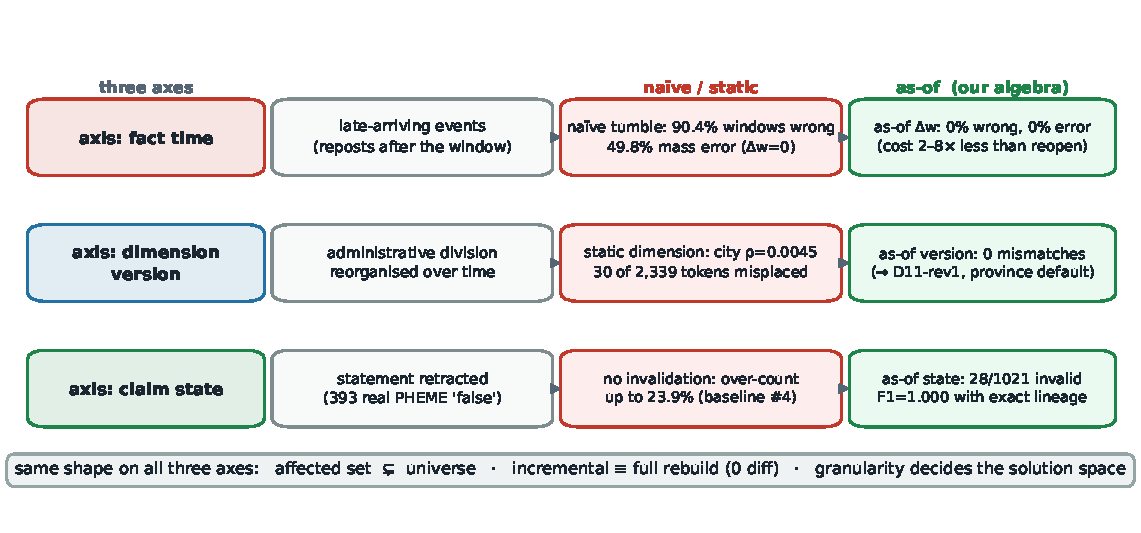
\includegraphics[width=0.88\columnwidth]{fig2_three_axis_asof.pdf}
\caption{Three axes, one shape. Each axis admits a na\"ive/static reading and
an as-of reading; the numbers are the measured outcomes of
\S7.2--\S7.4. All three share the same structure: the affected set is
a small fraction of the universe, incremental maintenance is bit-identical to
full rebuild, and representation granularity decides the solution space.}
\label{sfig:axes}
\end{figure}
